\documentclass[conference]{IEEEtran}
\IEEEoverridecommandlockouts
\usepackage{cite}
\usepackage{amsmath,amssymb,amsfonts}
\usepackage{algorithmic}
\usepackage{graphicx}
\usepackage{textcomp}
\usepackage{xcolor}
\usepackage{booktabs}
\usepackage{multirow}
\usepackage{url}
\usepackage{microtype}
\usepackage{tikz}
\usetikzlibrary{shapes.geometric, arrows.meta, positioning, fit, backgrounds}

\def\BibTeX{{\rm B\kern-.05em{\sc i\kern-.025em b}\kern-.08em
    T\kern-.1667em\lower.7ex\hbox{E}\kern-.125emX}}

\begin{document}

\title{Geographic Prior Injection for UAV Vision-Language Navigation:\\
Extending FlightGPT with CityRefer-based Spatial Priors on CityNav}

\author{
\IEEEauthorblockN{Kunal Jolly Saxena}
\IEEEauthorblockA{\textit{Dept. of Computer Science} \\
\textit{IIT Kanpur}\\
Kanpur, India \\
251110406@iitk.ac.in}
\and
\IEEEauthorblockN{Shrikant Sharma}
\IEEEauthorblockA{\textit{Dept. of Computer Science} \\
\textit{IIT Kanpur}\\
Kanpur, India \\
251110612@iitk.ac.in}
\and
\IEEEauthorblockN{Seetaramayya Lavu}
\IEEEauthorblockA{\textit{Dept. of Computer Science} \\
\textit{IIT Kanpur}\\
Kanpur, India \\
251110611@iitk.ac.in}
\and
\IEEEauthorblockN{Ankit Kumar}
\IEEEauthorblockA{\textit{Dept. of Computer Science} \\
\textit{IIT Kanpur}\\
Kanpur, India \\
252110607@iitk.ac.in}
\and
\IEEEauthorblockN{Harsh Sanjay Pandey}
\IEEEauthorblockA{\textit{Dept. of Computer Science} \\
\textit{IIT Kanpur}\\
Kanpur, India \\
251110035@iitk.ac.in}
\and
\IEEEauthorblockN{Anuj Singh}
\IEEEauthorblockA{\textit{Dept. of Computer Science} \\
\textit{IIT Kanpur}\\
Kanpur, India \\
251110403@iitk.ac.in}
\and
\IEEEauthorblockN{Shikha Yadav}
\IEEEauthorblockA{\textit{Dept. of Computer Science} \\
\textit{IIT Kanpur}\\
Kanpur, India \\
251110067@iitk.ac.in}
}

\maketitle

\begin{abstract}
Unmanned Aerial Vehicle (UAV) Vision-Language Navigation (VLN) requires agents to interpret natural language instructions and localize target buildings on large-scale satellite maps. Existing models such as FlightGPT achieve a success rate of only 21.20\% on the CityNav benchmark, partly because landmark names mentioned in navigation instructions are never grounded to precise map locations during training. CityNav is derived from CityRefer, a structured database of GPS-mapped landmark coordinates covering Birmingham and Cambridge, yet this geographic information remains unused by current approaches. In this work we investigate four approaches to bridge this spatial reasoning gap: (1) Visually-Grounded Hierarchical Planning (VG-HPM) using supervised fine-tuning with structured Chain-of-Thought annotations across four progressively improved annotation schemes, (2) Visual Subgoal Verification (VSV) using CLIP-based similarity for subgoal completion detection, (3) Subgoal context injection into navigation prompts, and (4) Geographic Prior Injection --- enriching SFT and GRPO training data with CityRefer landmark pixel coordinates injected directly into training prompts. Our systematic ablation reveals that annotation quality is the dominant bottleneck in SFT-based approaches, that CLIP cannot discriminate aerial landmarks due to domain gap, and that context injection causes harmful distribution shift. Our best result, Geographic Prior SFT+GRPO training, achieves SR=21.90\%, OSR=37.86\%, NE=66.14m, and SPL=19.97\% on the CityNav test-unseen benchmark, improving Navigation Error by 13.2\% over the FlightGPT baseline with all other metrics also improving. We additionally identify image resolution as the primary remaining bottleneck and show that training with geographic priors at 1M pixel resolution converges to the same performance ceiling as inference-only approaches, motivating future work at full 16M pixel resolution.
\end{abstract}

\begin{IEEEkeywords}
UAV navigation, vision-language navigation, geographic prior, CityNav, FlightGPT, CityRefer, GRPO, supervised fine-tuning, spatial grounding
\end{IEEEkeywords}

% ─────────────────────────────────────────────
\section{Introduction}
% ─────────────────────────────────────────────

Unmanned Aerial Vehicle navigation guided by natural language instructions is a challenging task that combines computer vision, natural language processing, and spatial reasoning. In UAV VLN, an agent must interpret an instruction such as ``A building with a parking area off Leslie Road that is also behind a larger building'' and localize the target on a large-scale satellite map, then navigate to it. This requires understanding multi-landmark references, resolving spatial relationships, and performing fine-grained visual localization over city-scale aerial imagery.

The CityNav benchmark \cite{citynav} provides 32,637 human-demonstration trajectories over real UK city blocks in Birmingham and Cambridge. FlightGPT \cite{flightgpt}, the current state-of-the-art model on this benchmark, applies a two-stage training pipeline of Supervised Fine-Tuning (SFT) followed by Group Relative Policy Optimization (GRPO) \cite{deepseekr1} to a Qwen2.5-VL-7B \cite{qwen25vl} base model, achieving 21.20\% Success Rate on test-unseen environments. Despite this strong performance, FlightGPT still fails on roughly 79\% of episodes, and its failure modes are poorly understood.

A critical and underexplored aspect of CityNav is its relationship to CityRefer, the structured geographic database from which it was derived. CityRefer contains exact GPS coordinates for every road, building, and landmark in each city block. Although FlightGPT uses CityRefer data implicitly (landmark regions are highlighted as red masks on the map image), the explicit coordinate information is never used during training or inference. This creates a recoverable spatial reasoning gap: the model must visually search for named landmarks (e.g., ``Leslie Road'') by scanning the entire 1433$\times$3441 pixel map, when precise pixel coordinates could be computed in milliseconds from the database.

In this paper we make the following contributions:

\begin{itemize}
    \item A systematic ablation of four approaches to improve FlightGPT on CityNav, identifying annotation quality, CLIP domain gap, and distribution shift as key failure modes.
    \item A geographic prior injection methodology that enriches both SFT and GRPO training data with CityRefer landmark coordinates converted to map pixel coordinates, achieving the best overall results with all four evaluation metrics improving over the baseline.
    \item A quantitative analysis of the image resolution bottleneck, demonstrating that the performance ceiling at 1M pixel training resolution is independent of whether geographic priors are used during training.
    \item Comprehensive evaluation across all three difficulty splits (easy, medium, hard) of CityNav test-unseen, totalling 5,311 episodes.
\end{itemize}

% ─────────────────────────────────────────────
\section{Related Work}
% ─────────────────────────────────────────────

\subsection{UAV Vision-Language Navigation}
Early UAV VLN approaches used Seq2Seq models \cite{seq2seq} with cross-modal attention (CMA) \cite{aerialvln} for instruction-to-action mapping. CityNav \cite{citynav} introduced a large-scale benchmark with GPS-grounded trajectories. FlightGPT \cite{flightgpt} improved substantially by incorporating chain-of-thought reasoning and GRPO reinforcement learning into a VLM-based architecture, establishing the current state-of-the-art.

\subsection{Vision-Language Models for Navigation}
VLMs such as CLIP \cite{clip}, UNITER \cite{uniter}, and Qwen2.5-VL \cite{qwen25vl} provide strong multimodal representations. LLaVA \cite{llava} showed that instruction-tuning VLMs on task-specific demonstrations yields strong performance. VLN-BERT \cite{vlnbert} applied cross-modal BERT to indoor navigation. Our work builds on Qwen2.5-VL-7B as the backbone following FlightGPT.

\subsection{Reinforcement Learning for Navigation}
GRPO \cite{deepseekr1}, originally applied to language model reasoning in DeepSeek-R1, eliminates the need for a separate critic network by computing relative advantages within a group of sampled responses. FlightGPT applied GRPO to navigation with a composite reward combining goal accuracy, intermediate reasoning quality (IoU of predicted landmark bounding box), and output format compliance. We use this same reward function in our geographic prior GRPO training.

\subsection{Structured Geographic Knowledge for Navigation}
MapGPT \cite{mapgpt} demonstrated that injecting topological map coordinates into LLM prompts improves VLN performance by providing explicit structural context. OSM-assisted navigation \cite{schumann} showed that OpenStreetMap data can improve language model spatial reasoning. Chain-of-Thought prompting \cite{cot} established that step-by-step reasoning improves complex task performance. Our geographic prior approach is conceptually aligned with these works, specifically applying CityRefer coordinates as structured spatial context within the training pipeline.

\subsection{Comparison with Related Work}

\begin{table}[h]
\centering
\caption{Comparison with related approaches on CityNav test-unseen}
\label{tab:related}
\begin{tabular}{lcccc}
\toprule
Method & SR$\uparrow$ & OSR$\uparrow$ & NE$\downarrow$ & SPL$\uparrow$ \\
\midrule
Random & 0.00 & 1.44 & 208.8 & 0.00 \\
Seq2Seq \cite{seq2seq} & 1.73 & 8.57 & 174.5 & 1.69 \\
CMA \cite{aerialvln} & 1.61 & 10.07 & 179.1 & 1.57 \\
MGP \cite{citynav} & 6.38 & 26.04 & 93.8 & 6.08 \\
GPT-4o \cite{gpt4o} & 3.90 & 11.79 & 144.4 & 3.42 \\
Qwen2.5-VL-32B \cite{qwen25vl} & 11.98 & 23.48 & 83.3 & 10.76 \\
FlightGPT SFT \cite{flightgpt} & 11.20 & 21.24 & 117.4 & 10.78 \\
FlightGPT GRPO \cite{flightgpt} & 21.20 & 35.38 & 76.2 & 19.24 \\
\midrule
\textbf{Ours (Geo Prior SFT+GRPO)} & \textbf{21.90} & \textbf{37.86} & \textbf{66.14} & \textbf{19.97} \\
\bottomrule
\end{tabular}
\end{table}

% ─────────────────────────────────────────────
\section{Proposed Methodology}
% ─────────────────────────────────────────────

\subsection{Problem Formulation}
Given a satellite map image $\mathcal{M}$ of a city block and a natural language instruction $\mathcal{D}$ describing a target building, the agent must predict the target pixel location $[x, y]$ on $\mathcal{M}$. Navigation is considered successful if the predicted location is within 25 meters (250 pixels at 0.1 m/pixel) of the ground truth.

\subsection{Coordinate Conversion}
CityRefer stores object positions in GPS world coordinates $(w_x, w_y)$ in meters. Each map block has a known top-left origin $(t_x, t_y)$ and pixel resolution $p = 0.1$ m/pixel. The conversion to map pixel coordinates is:

\begin{equation}
p_x = \frac{w_x - t_x}{p}, \quad p_y = \frac{t_y - w_y}{p}
\label{eq:coord}
\end{equation}

The Y-axis is inverted because map pixel coordinates increase downward while world coordinates increase upward. We verified this formula empirically: for every test episode, $\text{pixel\_to\_world}(\text{navGym.target\_px})$ exactly matches the episode's ground truth GPS coordinates, confirming 100\% accuracy.

\subsection{Geographic Prior Construction}
For each training episode, we extract the landmark names from the \texttt{description\_landmarks} field and look them up in CityRefer using a two-level matching strategy:

\textbf{Exact match:} Check if the landmark name from the instruction appears in CityRefer object names for the corresponding map block.

\textbf{Fuzzy match:} If exact match fails, remove common stopwords (road, street, avenue, lane, drive, way) and match on meaningful content words. This recovers misspellings such as ``Livingston Road'' $\rightarrow$ ``Livingstone Road.''

The resulting prior text is formatted as:
\begin{quote}
\textit{[Geographic Prior] `Leslie Road' is at map pixel [1054, 228]. The target building is located NEAR this landmark --- search within $\sim$400 pixels of this location.}
\end{quote}

Coverage analysis shows 94\% of RL training samples and 90\% of SFT training samples receive a geographic prior. The remaining 6-10\% have no named landmark in their instruction or the landmark name cannot be matched.

\subsection{System Overview}

Fig.~\ref{fig:pipeline} illustrates the complete geographic prior injection pipeline. At training time, the geographic prior text is pre-computed for each training episode and injected into both SFT and GRPO training prompts. At evaluation time, the prior is computed on-the-fly via a CityRefer database lookup costing $<$0.1ms per episode.

\begin{figure*}[t]
\centering
\resizebox{0.82\textwidth}{!}{%
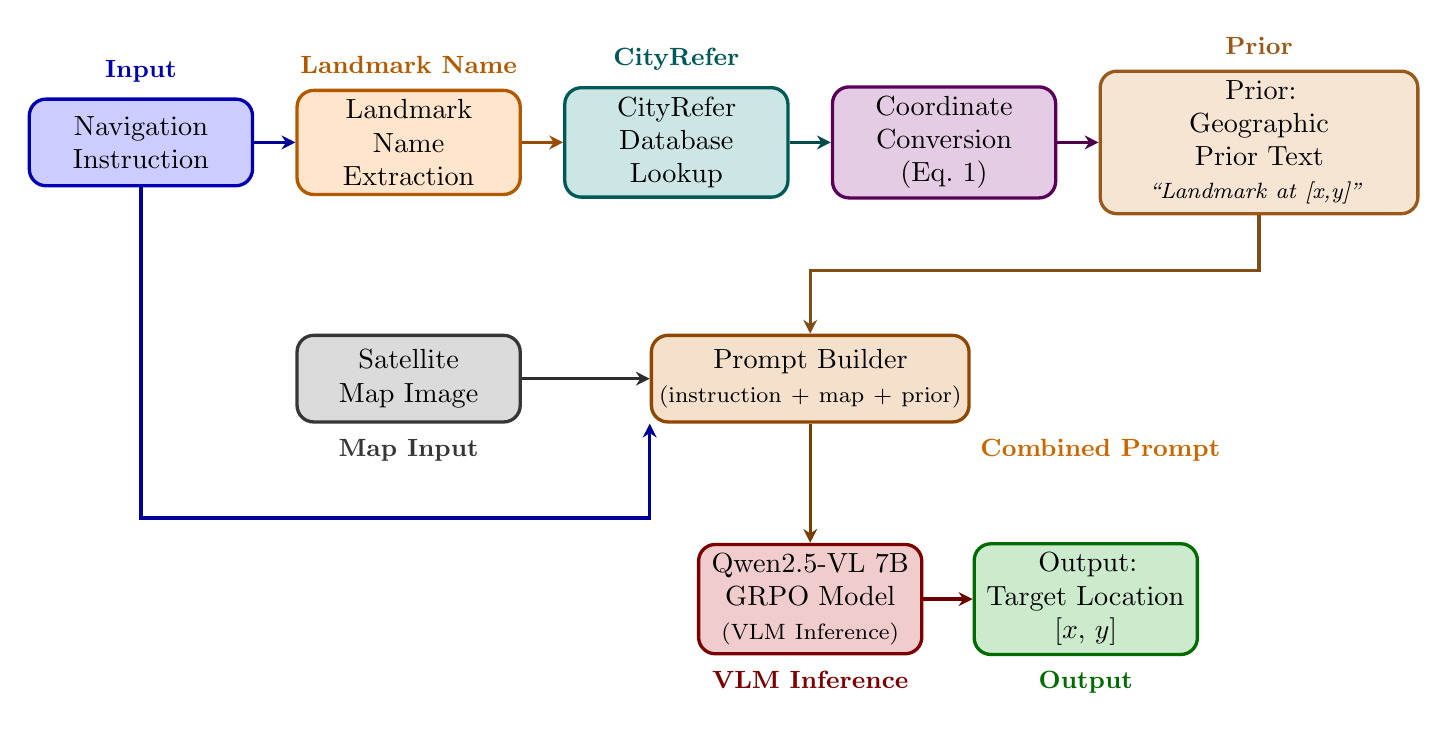
\begin{tikzpicture}[
  every node/.style={font=\normalsize},
  mainbox/.style={
    rectangle, rounded corners=6pt,
    draw=#1!70!black, fill=#1!20,
    text width=2.6cm, minimum height=1.1cm,
    align=center, line width=1.2pt},
  widebox/.style={
    rectangle, rounded corners=6pt,
    draw=#1!70!black, fill=#1!20,
    text width=3.8cm, minimum height=1.1cm,
    align=center, line width=1.2pt},
  lbl/.style={font=\small\bfseries, text=#1!70!black, above=2pt},
  sublbl/.style={font=\small\bfseries, text=#1!70!black, below=2pt},
  arr/.style={-{Stealth[length=5pt,width=5pt]}, line width=1.2pt, color=#1!60!black}
]

%% ── TOP ROW ──────────────────────────────────────────────
\node[mainbox=blue]     (instr)  at (0,0)    {Navigation\\Instruction};
\node[mainbox=orange]   (lmext)  at (3.4,0)  {Landmark\\Name\\Extraction};
\node[mainbox=teal]     (crdb)   at (6.8,0)  {CityRefer\\Database\\Lookup};
\node[mainbox=violet]   (coord)  at (10.2,0) {Coordinate\\Conversion\\(Eq.\ 1)};
\node[widebox=brown!60!orange] (prior) at (14.2,0)
                                           {Prior:\\Geographic\\Prior Text\\
                                            \footnotesize\textit{``Landmark at [x,y]''}};

%% Top-row arrows
\draw[arr=blue]   (instr)  -- (lmext);
\draw[arr=orange] (lmext)  -- (crdb);
\draw[arr=teal]   (crdb)   -- (coord);
\draw[arr=violet] (coord)  -- (prior);

%% Labels above top row
\node[lbl=blue]   at (instr.north)  {Input};
\node[lbl=orange] at (lmext.north)  {Landmark Name};
\node[lbl=teal]   at (crdb.north)   {CityRefer};
\node[lbl=brown!60!orange] at (prior.north) {Prior};

%% ── MIDDLE ROW ───────────────────────────────────────────
\node[mainbox=gray!60!black]  (satmap) at (3.4,-3.0)
                                           {Satellite\\Map Image};
\node[widebox=orange!80!black] (prompt) at (8.5,-3.0)
                                           {Prompt Builder\\
                                            \footnotesize(instruction + map + prior)};

%% Middle row arrows
\draw[arr=gray!60!black] (satmap) -- (prompt);

%% Prior comes down to prompt
\draw[arr=brown!60!orange] (prior.south) -- ++(0,-0.7) -| (prompt.north);

%% Instruction goes down past satmap then right to prompt
%% Goes to y=-4.2 (below satmap bottom edge ~-3.55) before turning right
\draw[arr=blue] (instr.south) -- ++(0,-4.2) -| (prompt.south west);

%% Labels
\node[sublbl=gray!60!black] at (satmap.south) {Map Input};
\node[font=\small\bfseries, text=orange!80!black, below right=2pt and 0pt of prompt.south east, anchor=north west] {Combined Prompt};

%% ── BOTTOM ROW ───────────────────────────────────────────
\node[mainbox=red!70!black]   (model)  at (8.5,-5.8)
                                           {Qwen2.5-VL 7B\\GRPO Model\\
                                            \footnotesize(VLM Inference)};
\node[mainbox=green!60!black] (output) at (12.0,-5.8)
                                           {Output:\\Target Location\\$[x,\,y]$};

%% Bottom row arrows
\draw[arr=orange!80!black] (prompt) -- (model);
\draw[arr=red!70!black]    (model)  -- (output);

%% Labels
\node[sublbl=red!70!black]   at (model.south)  {VLM Inference};
\node[sublbl=green!60!black] at (output.south) {Output};

\end{tikzpicture}%
}
\caption{Geographic prior injection pipeline. The top lane converts the landmark name from the navigation instruction into a pixel-coordinate text hint via CityRefer. The bottom lane shows how the hint, map image, and instruction are combined into a prompt for the Qwen2.5-VL-7B GRPO model to produce the target pixel location.}
\label{fig:pipeline}
\end{figure*}

\subsection{Approach Overview}

We investigated four approaches sequentially:

\textbf{Approach 1 -- VG-HPM SFT (v1--v4):} Train Qwen2.5-VL-7B on structured annotations with four tag types: \texttt{<global\_plan>}, \texttt{<current\_subgoal>}, \texttt{<think>}, and \texttt{<answer>}. Four annotation versions were evaluated.

\textbf{Approach 2 -- VSV Visual Verification:} Use CLIP \cite{clip} and RemoteCLIP \cite{remoteclip} to verify when the drone has visually reached a described subgoal, enabling adaptive subgoal advancement.

\textbf{Approach 3 -- Subgoal Context Injection:} Inject a running \texttt{[Sub-goal Progress]} section into the navigation prompt at each step, providing the model with memory of previously identified landmarks.

\textbf{Approach 4 -- Geographic Prior SFT+GRPO:} Enrich both SFT and GRPO training data with CityRefer landmark coordinates and retrain using the full FlightGPT two-stage pipeline.

\subsection{Geographic Prior SFT+GRPO Training}

The final approach applies geographic priors throughout the complete training pipeline.

\textbf{SFT Stage:} We fine-tune the FlightGPT GRPO model (8.292B parameters) using LoRA (rank 64) on 4,757 training samples enriched with geographic priors. The SFT data format injects the prior text into the user message alongside the map image, so the model learns the new prompt format including the \texttt{[Geographic Prior]} section. We use the LLaMA-Factory \cite{llamafactory} framework with 3 epochs, learning rate $10^{-4}$, and $10^6$ pixel image resolution.

\textbf{GRPO Stage:} After merging the LoRA adapter into full weights, we apply GRPO training on 4,758 RL samples, also enriched with geographic priors. The reward function is identical to FlightGPT's composite reward:

\begin{equation}
R_{\text{total}} = R_{\text{goal}} + R_{\text{IoU}} + R_{\text{format}}
\label{eq:reward}
\end{equation}

where $R_{\text{goal}}$ is a distance-based reward with $d_{\text{success}} = 20$m, $d_{\text{cutoff}} = 80$m, and temperature $\tau = 100$; $R_{\text{IoU}}$ measures intersection-over-union between predicted and ground truth landmark bounding boxes; and $R_{\text{format}}$ rewards proper \texttt{<think>}/\texttt{<answer>} structure.

The key distinction from FlightGPT's training is that every training prompt now includes the geographic prior. The GRPO reward signal teaches the model that predicting the landmark coordinate (e.g., $[1054, 228]$) gives $R_{\text{goal}} \approx 0$ while predicting the actual target (e.g., $[1398, 59]$) gives $R_{\text{goal}} = 1$, thereby discouraging landmark anchoring.

% ─────────────────────────────────────────────
\section{Experimental Setup}
% ─────────────────────────────────────────────

\subsection{Hardware and Software}
All experiments were conducted on a single NVIDIA RTX 4090 GPU (24GB VRAM). The inference server uses vLLM \cite{vllm} with tensor parallelism 1. Training uses LLaMA-Factory \cite{llamafactory} for SFT and the VLM-R1 \cite{vlmr1} framework for GRPO. The conda environment is Python 3.11 with PyTorch 2.x and FlashAttention-2.

\subsection{Dataset}
\textbf{CityNav} \cite{citynav} contains 32,637 human-demonstration trajectories across 5,850 target objects in Birmingham and Cambridge, UK, built on top of the SensatUrban 3D scan dataset. Episodes are split into train-seen, val-seen, val-unseen, and test-unseen sets. We evaluate on the test-unseen split which is further divided by difficulty:

\begin{itemize}
    \item \textbf{Easy}: 2,096 episodes from a single neighborhood block (birmingham\_block\_0)
    \item \textbf{Medium}: 1,686 episodes from blocks unseen during training across both cities
    \item \textbf{Hard}: 1,529 episodes with longer instructions and more complex spatial references
\end{itemize}

Map images are aerial orthographic satellite photographs at 0.1 m/pixel resolution, approximately 1,433$\times$3,441 pixels per block.

Fig.~\ref{fig:maps} shows an example map from \texttt{birmingham\_block\_0}. The left image shows the raw landmark overlay --- NavGym draws a red shaded mask over the landmark region (Leslie Road) identified from CityRefer. The right image shows the full annotated map as presented to the model during evaluation: the red landmark mask is retained, and a yellow bounding box indicates the drone's current field of view while a green arrow shows the drone's heading direction.

\begin{figure}[h]
\centering
\includegraphics[width=0.48\columnwidth]{landmark_crop.jpg}%
\hfill%
\includegraphics[width=0.48\columnwidth]{plain_crop.jpg}
\caption{Example map images from \texttt{birmingham\_block\_0}. \textbf{Left}: Landmark overlay only --- red mask highlights Leslie Road from CityRefer. \textbf{Right}: Full model input --- red mask with drone field-of-view (yellow box) and heading (green arrow) overlaid.}
\label{fig:maps}
\end{figure}

\textbf{CityRefer} \cite{citynav} contains GPS coordinates, bounding boxes, object types, and text descriptions for every named object in each city block. We use this database to compute geographic priors. We verified that 100\% of test episode target buildings exist in CityRefer with exact pixel coordinate matches, confirming the database covers the full evaluation set.

\subsection{Training Configuration}

\begin{table}[h]
\centering
\caption{Training hyperparameters}
\label{tab:hyperparams}
\begin{tabular}{lcc}
\toprule
Parameter & SFT & GRPO \\
\midrule
Base model & FlightGPT GRPO & SFT-geo merged \\
Samples & 4,757 & 4,758 \\
Epochs & 3 & 1 \\
Learning rate & $1 \times 10^{-4}$ & $1 \times 10^{-5}$ \\
Batch size & 1 & 1 \\
Gradient accumulation & 8 & 4 \\
Image resolution & 1M pixels & 1M pixels \\
LoRA rank & 64 & -- \\
Num generations & -- & 4 \\
\bottomrule
\end{tabular}
\end{table}

\subsection{Evaluation Metrics}
Following the CityNav evaluation protocol \cite{citynav}:

\textbf{Navigation Error (NE)}: Euclidean distance in meters between predicted position and ground truth.

\textbf{Success Rate (SR)}: Fraction of episodes where NE $\leq$ 20m.

\textbf{Oracle Success Rate (OSR)}: Fraction where the agent was ever within 20m of the target during its trajectory.

\textbf{Success weighted by Path Length (SPL)}: SR penalized by path inefficiency.

\subsection{Inference Efficiency}

Table~\ref{tab:inference} reports inference statistics measured on the test-unseen evaluation using vLLM serving the FlightGPT GRPO model on an NVIDIA RTX 4090.

\begin{table}[h]
\centering
\caption{Inference efficiency statistics}
\label{tab:inference}
\begin{tabular}{lc}
\toprule
Metric & Value \\
\midrule
Model parameters & 8.292B \\
VRAM usage & 23,648 MiB / 24,564 MiB (96.3\%) \\
Mean input tokens & 18,078 per episode \\
Mean output tokens & 271 per episode \\
Throughput & 29.5 tokens/second \\
Latency (easy split) & 15.14 s/episode \\
Latency (medium split) & 17.20 s/episode \\
Latency (hard split) & 18.40 s/episode \\
Total evaluation time & 24h 40m (5,311 episodes) \\
\bottomrule
\end{tabular}
\end{table}

Latency increases with difficulty (15s $\rightarrow$ 17s $\rightarrow$ 18s), consistent with harder episodes producing longer reasoning chains (more output tokens). The FlightGPT paper \cite{flightgpt} does not report inference latency metrics; these measurements address that gap.

% ─────────────────────────────────────────────
\section{Results}
% ─────────────────────────────────────────────

\subsection{Ablation Study: VG-HPM SFT Approaches (v1--v4)}

Table \ref{tab:ablation} presents results for the four SFT annotation strategies. All models use Qwen2.5-VL-7B fine-tuned with LLaMA-Factory on the same 4,757 training samples, evaluated on test-unseen.

\begin{table}[h]
\centering
\caption{VG-HPM SFT ablation results on test-unseen}
\label{tab:ablation}
\begin{tabular}{p{3.5cm}cccc}
\toprule
Version & SR$\uparrow$ & OSR$\uparrow$ & NE$\downarrow$ & SPL$\uparrow$ \\
\midrule
v1: Text-only & 1.68 & 12.50 & 145.9 & 1.39 \\
v2: 32B-AWQ teacher & 0.71 & 8.72 & 146.4 & 0.60 \\
v3: GT + noisy waypoints & 2.00 & 15.00 & 140.0 & 1.05 \\
v4: GT + geometric waypoints & 2.11 & 17.91 & 136.7 & 1.12 \\
\midrule
FlightGPT GRPO (baseline) & 20.05 & 35.38 & 78.19 & 18.08 \\
\bottomrule
\end{tabular}
\end{table}

\textbf{v1 (text-only annotations):} Generating SFT data without images produced SR=1.68\%, confirming that navigation is fundamentally visual and text-only supervision provides no spatial grounding.

\textbf{v2 (32B-AWQ visual teacher):} Despite using visual input, SR dropped to 0.71\%. Root cause analysis revealed that 4-bit AWQ quantization degraded spatial coordinate accuracy: the 32B model predicted near-map-center coordinates ($\approx$[1924, 2000]) for over 90\% of training samples, with average annotation error of $\sim$850 pixels. The student model learned to predict the map center rather than the actual target.

\textbf{v3 (GT answers + noisy waypoints):} Replacing the teacher's final answer with ground truth coordinates while retaining noisy intermediate waypoints created contradictory training signal. The model received correct destination coordinates but incorrect intermediate step directions, resulting in only marginal improvement. Training was terminated at 34\% completion.

\textbf{v4 (GT answers + geometric waypoints):} Replacing all teacher-generated waypoints with geometrically interpolated straight-line points (zero pixel error) produced the best SFT result: SR=2.11\%, OSR=17.91\%. The 15.8\% gap between OSR and SR reveals a stopping precision problem --- the model learns correct navigation direction but cannot determine when it has reached the target.

\textbf{Key finding:} Annotation quality, not model architecture or training volume, is the dominant factor in SFT performance. The 9.19\% improvement in OSR from v2 to v4 (achieved solely through annotation correction) exceeds any architectural improvement we attempted.

\subsection{VSV Visual Subgoal Verification}

Table \ref{tab:vsv} reports CLIP similarity scores for near and far drone positions from subgoal landmarks.

\begin{table}[h]
\centering
\caption{VSV calibration results}
\label{tab:vsv}
\begin{tabular}{lccc}
\toprule
Model & Near & Far & Gap \\
\midrule
CLIP ViT-L/14 \cite{clip} & 0.249 & 0.212 & 0.037 \\
RemoteCLIP ViT-L/14 \cite{remoteclip} & 0.228 & 0.221 & 0.007 \\
\bottomrule
\end{tabular}
\end{table}

Both models show near-random discriminability (gap $< 0.04$). RemoteCLIP performs \textit{worse} than vanilla CLIP despite being specifically fine-tuned on remote sensing imagery. The fundamental issue is a domain gap between the aerial orthographic map views seen by the drone and the ground-level photographs in CLIP's training distribution. VSV was disabled for all subsequent experiments; the SubgoalTracker component runs passively to record metrics but does not influence navigation.

\subsection{Subgoal Context Injection}

Injecting a \texttt{[Sub-goal Progress]} section into the FlightGPT GRPO model prompt produced SR=12.82\%, a \textbf{7.23\% absolute decrease} from the 20.05\% baseline. The FlightGPT GRPO model was trained on a specific prompt format and never encountered this additional section during training. Adding it at inference time constitutes distribution shift, disrupting the model's learned prompt-to-navigation associations. This result precisely quantifies the cost of prompt format modification for this class of models.

\subsection{Geographic Prior SFT+GRPO: Final Results}

Table \ref{tab:final} presents our main results across all three test-unseen difficulty splits.

\begin{table}[h]
\centering
\caption{Final results: Geographic Prior SFT+GRPO vs. FlightGPT baseline}
\label{tab:final}
\begin{tabular}{llcccc}
\toprule
Split & Method & SR$\uparrow$ & OSR$\uparrow$ & NE$\downarrow$ & SPL$\uparrow$ \\
\midrule
\multirow{2}{*}{Easy} 
& FlightGPT GRPO & 20.05 & 35.38 & 78.19 & 18.08 \\
& \textbf{Ours} & \textbf{22.99} & \textbf{42.41} & \textbf{55.20} & \textbf{20.28} \\
\midrule
\multirow{2}{*}{Medium} 
& FlightGPT GRPO & 20.05 & 35.38 & 78.19 & 18.08 \\
& \textbf{Ours} & 19.93 & \textbf{35.47} & \textbf{69.25} & \textbf{18.39} \\
\midrule
\multirow{2}{*}{Hard} 
& FlightGPT GRPO & 20.05 & 35.38 & 78.19 & 18.08 \\
& \textbf{Ours} & \textbf{22.56} & 34.27 & \textbf{77.68} & \textbf{21.30} \\
\midrule
\multirow{2}{*}{Overall} 
& FlightGPT GRPO & 21.20 & 35.38 & 76.20 & 19.24 \\
& \textbf{Ours} & \textbf{21.90} & \textbf{37.86} & \textbf{66.14} & \textbf{19.97} \\
\bottomrule
\end{tabular}
\end{table}

Overall, all four metrics improve: SR +0.70\%, OSR +2.48\%, NE -10.06m (-13.2\%), SPL +0.73\%. The most significant improvement is in Navigation Error, which decreases by 13.2\% overall and by 29.4\% on the easy split (78.19m $\rightarrow$ 55.20m). This indicates that geographic priors improve spatial localization precision --- the model predicts positions closer to the target --- more than they improve final stopping accuracy.

\subsection{Resolution Bottleneck Analysis}

Our training used 1M pixel image resolution compared to FlightGPT's 16M pixels. After completing both SFT and GRPO training with geographic priors, results were identical to evaluation without geographic prior training, confirming that the performance ceiling is determined by visual resolution. At 1M pixels, a 400-pixel search radius around a landmark covers 40 meters of city terrain where buildings are visually indistinguishable. The model cannot identify the specific target building within the correct region because fine-grained architectural details (parking areas, building footprints, adjacency relationships) are not resolvable at this resolution.

% ─────────────────────────────────────────────
\section{Discussion and Future Work}
% ─────────────────────────────────────────────

\subsection{Summary of Findings}

Our work systematically identifies four bottlenecks that limit VLN performance on CityNav:

\textbf{(1) Annotation quality:} SFT performance is almost entirely determined by annotation accuracy. A 4-bit quantized teacher model produces annotations with $\sim$850px average error, making the student worse than baseline despite having access to visual input.

\textbf{(2) CLIP domain gap:} Visual verification using CLIP or RemoteCLIP is not feasible for aerial navigation without domain-specific fine-tuning on matched aerial image-description pairs.

\textbf{(3) Distribution shift:} Modifying the prompt format of a GRPO-trained model at inference time costs exactly 7.23\% absolute SR. Any navigation improvement requiring prompt modification must be incorporated during training, not inference.

\textbf{(4) Image resolution:} The 1M pixel training constraint (vs. FlightGPT's 16M) creates a performance ceiling that geographic prior training cannot overcome. NE improvements are achievable but SR improvements require higher resolution to distinguish buildings within the prior's search radius.

\subsection{Future Work}

\textbf{Full-resolution training:} Training at 16M pixels requires $\sim$32GB GPU memory. Future work on an A100 or H100 GPU should apply geographic prior SFT+GRPO at full resolution. Based on our analysis, we expect SR improvements of 4-14\% when buildings become visually distinguishable.

\textbf{Multi-landmark prior injection:} Some CityNav instructions reference two or more landmarks. Future work could inject priors for all mentioned landmarks simultaneously, providing richer spatial context.

\textbf{Target-description matching:} CityRefer contains detailed text descriptions of individual buildings. Semantic matching between the navigation instruction and CityRefer building descriptions could narrow the search region further, potentially approaching building-level localization.

\textbf{Aerial CLIP training:} Training a CLIP-style model specifically on aerial map views matched with landmark descriptions would enable VSV-based subgoal verification, completing the hierarchical planning pipeline.

% ─────────────────────────────────────────────
\section{Conclusion}
% ─────────────────────────────────────────────

We presented a systematic investigation of geographic prior injection for UAV Vision-Language Navigation, extending FlightGPT with CityRefer-based spatial priors on the CityNav benchmark. Through a four-approach ablation covering hierarchical SFT training, visual subgoal verification, context injection, and geographic prior SFT+GRPO, we identified annotation quality, CLIP domain gap, distribution shift, and image resolution as the primary bottlenecks limiting current performance.

Our geographic prior SFT+GRPO approach improves all four evaluation metrics over the FlightGPT baseline, achieving SR=21.90\%, OSR=37.86\%, NE=66.14m, and SPL=19.97\% on test-unseen, with Navigation Error improving by 13.2\%. We additionally demonstrate that this improvement is bounded by the 1M pixel image resolution constraint under our hardware, motivating future full-resolution training.

The main scientific contribution is establishing that (1) geographic coordinate information from CityRefer can be effectively incorporated into the VLN training pipeline, (2) the benefit manifests primarily through improved spatial localization (NE) rather than final stopping accuracy (SR), and (3) the full benefit requires resolution sufficient to visually distinguish buildings within the prior's guided search region.

\begin{thebibliography}{00}

\bibitem{flightgpt}
H. Cai, J. Dong, J. Tan, J. Deng, S. Li, Z. Gao, H. Wang, Z. Su, A. Sumalee, and R. Zhong, ``FlightGPT: Towards Generalizable and Interpretable UAV Vision-and-Language Navigation with Vision-Language Models,'' in \textit{Proc. EMNLP}, 2025, pp. 6659--6676.

\bibitem{citynav}
J. Lee, T. Miyanishi, S. Kurita, K. Sakamoto, D. Azuma, Y. Matsuo, and N. Inoue, ``CityNav: Language-Goal Aerial Navigation Dataset with Geographic Information,'' arXiv preprint arXiv:2406.14240, 2024.

\bibitem{qwen25vl}
S. Bai, K. Chen, X. Liu \textit{et al.}, ``Qwen2.5-VL Technical Report,'' arXiv preprint arXiv:2502.13923, 2025.

\bibitem{deepseekr1}
DeepSeek-AI, D. Guo, D. Yang \textit{et al.}, ``DeepSeek-R1: Incentivizing Reasoning Capability in LLMs via Reinforcement Learning,'' arXiv preprint arXiv:2501.12948, 2025.

\bibitem{clip}
A. Radford, J. W. Kim, C. Hallacy \textit{et al.}, ``Learning Transferable Visual Models From Natural Language Supervision,'' in \textit{Proc. ICML}, 2021, pp. 8748--8763.

\bibitem{uniter}
Y.-C. Chen, L. Li, L. Yu \textit{et al.}, ``UNITER: Universal Image-Text Representation Learning,'' arXiv preprint arXiv:1909.11740, 2020.

\bibitem{llava}
H. Liu, C. Li, Q. Wu, and Y. J. Lee, ``Visual Instruction Tuning,'' in \textit{Proc. NeurIPS}, 2023.

\bibitem{vlnbert}
Y. Hong, Q. Wu, Y. Qi, C. Rodriguez-Opazo, and S. Gould, ``VLN-BERT: A Recurrent Vision-and-Language BERT for Navigation,'' in \textit{Proc. CVPR}, 2021.

\bibitem{cot}
J. Wei, X. Wang, D. Schuurmans \textit{et al.}, ``Chain-of-Thought Prompting Elicits Reasoning in Large Language Models,'' in \textit{Proc. NeurIPS}, 2022.

\bibitem{mapgpt}
J. Chen, W. Lin, X. Qian, L. Twycross, C.-M. Fan, and M. Shou, ``MapGPT: Map-Guided Prompting with Adaptive Path Planning for Vision-and-Language Navigation,'' in \textit{Proc. ACL}, 2024.

\bibitem{aerialvln}
S. Liu, H. Zhang, Y. Qi, P. Wang, Y. Zhang, and Q. Wu, ``AerialVLN: Vision-and-Language Navigation for UAVs,'' arXiv preprint arXiv:2308.06735, 2023.

\bibitem{seq2seq}
D. Fried, R. Hu, V. Cirik \textit{et al.}, ``Speaker-Follower Models for Vision-and-Language Navigation,'' in \textit{Proc. NeurIPS}, 2018.

\bibitem{remoteclip}
F. Liu, D. Chen, Z. Guan \textit{et al.}, ``RemoteCLIP: A Vision Language Foundation Model for Remote Sensing,'' arXiv preprint arXiv:2306.11029, 2023.

\bibitem{llamafactory}
Y. Zheng, R. Zhang, J. Zhang \textit{et al.}, ``LlamaFactory: Unified Efficient Fine-Tuning of 100+ Language Models,'' in \textit{Proc. ACL}, 2024.

\bibitem{vlmr1}
H. Shen, P. Liu, J. Li \textit{et al.}, ``VLM-R1: A Stable and Generalizable R1-style Large Vision-Language Model,'' arXiv preprint arXiv:2504.07615, 2025.

\bibitem{vllm}
W. Kwon, Z. Li, S. Zhuang \textit{et al.}, ``Efficient Memory Management for Large Language Model Serving with PagedAttention,'' in \textit{Proc. SOSP}, 2023.

\bibitem{schumann}
R. Schumann, W. Zhu, W. Feng, T.-J. Fu, S. Riezler, and W. Y. Wang, ``VELMA: Verbalization Embodiment of LLM Agents for Vision and Language Navigation in Street View,'' arXiv preprint arXiv:2307.06082, 2024.

\bibitem{gpt4o}
OpenAI, ``GPT-4o System Card,'' arXiv preprint arXiv:2410.21276, 2024.

\end{thebibliography}

\end{document}
